\documentclass[12pt, letterpaper]{article}

%++++++++++++++++++++++++++++++++++++++++
% Don't modify this section unless you know what you're doing!
\usepackage{tabularx} % Extra features for tabular environment
\usepackage{amssymb, amsfonts, amsmath, amsthm}  % Improve math presentation
\usepackage{graphicx} % Handles graphic inclusion
\usepackage[margin=1in,letterpaper]{geometry} % Sets margins
\usepackage{cite} % Manages citations
\usepackage[final]{hyperref} % Adds hyperlinks in the PDF
\usepackage{float} % Improved interface for floating objects
\usepackage{booktabs} % Enhanced table formatting
\usepackage{tikz} % Drawing package
\usepackage{fancyhdr} % Fancy header and footer
\usepackage{lastpage} % Reference to the last page
\usepackage{lipsum} % Generates filler text

\DeclareMathOperator*{\argmin}{arg\,min} % Defines \argmin
\DeclareMathOperator*{\argmax}{arg\,max} % Defines \argmax

\renewcommand*\contentsname{Table of Contents} % Title of contents list
\setlength{\headheight}{15pt}
\setlength{\footskip}{45pt}

\hypersetup{
    colorlinks=true,       % false: boxed links; true: colored links
    linkcolor=blue,        % color of internal links
    citecolor=blue,        % color of links to bibliography
    filecolor=magenta,     % color of file links
    urlcolor=blue          % color of URLs
}
%++++++++++++++++++++++++++++++++++++++++

% Title and Author Information
\title{\textbf{IEEE ITÜ RAS Teknik Ekip } \\  Rapor Şablonu} 
\author{
    \textbf{Your Name} \\
    Your Affiliation \\
    \texttt{your.email@example.com}
}
\date{\today} % Replace with a specific date if desired

% Abstract Text
\newcommand{\abstractText}{%
    In this report, we explore... % Replace with your actual abstract text
}

% Logo Paths
\newcommand{\lablogo}{images/ieee_ras_logo.png} % Path to the main logo
\newcommand{\footerlogo}{images/ieee_ras_logo.png} % Path to the footer logo

\begin{document}

\makeatletter
    \begin{titlepage}
        \begin{center}
            \vspace*{1cm}
            
            % IEEE RAS Logo
            \includegraphics[width=4cm]{\lablogo}\\[1cm]
            
            % Report Title
            {\LARGE \bfseries \@title}\\[2cm]
            
            % Author Information
            {\large
            \textbf{\@author} \\
            \@date
            }
            
            \vfill
            
            % Abstract
            \begin{abstract}
                \abstractText
            \end{abstract}
        \end{center}
        
        % Footer Logo
        \tikz [remember picture, overlay] %
        \node [shift={(-2.4cm,0.5cm)}] at (current page.south east) %
        [anchor=south east] %
        {\includegraphics[width=1cm]{\footerlogo}};
    \end{titlepage}
\makeatother

% Configure Header and Footer
\pagestyle{fancy}
\fancyhf{}
\rhead{\textbf{Your Report Title}}
\lfoot{Page \thepage\ of \pageref{LastPage}}
\rfoot{\includegraphics[width=1cm]{\footerlogo}}

\tableofcontents
\newpage

\section{Introduction}
Write your introduction section here

Example figure usage
\begin{figure}[H]
    \centering
    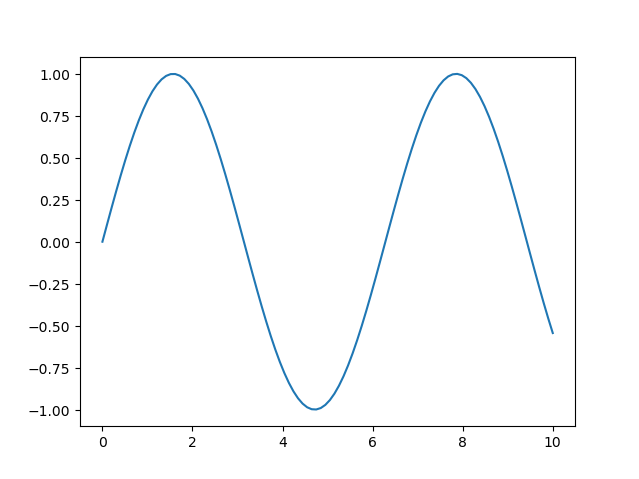
\includegraphics[width=0.5\textwidth]{images/sample_figure.png}
    \caption{Sample Figure}
    \label{fig:sample}
\end{figure}


\section{Methodology}
Write your methodology here

Example table usage
\begin{table}[H]
    \centering
    \begin{tabular}{|c|c|c|}
        \hline
        A & B & C \\ \hline
        1 & 2 & 3 \\ \hline
        4 & 5 & 6 \\ \hline
    \end{tabular}
    \caption{Sample Table}
    \label{tbl:sample}
\end{table}



\section{Results}
Explain and talk about your results here

Example list usage

    \begin{itemize}
        \item Point One
        \item Point Two
        \item Point Three
    \end{itemize}
    
    \begin{enumerate}
        \item First Item
        \item Second Item
        \item Third Item
    \end{enumerate}

\section{Conclusion}
Write your conclusion here
% References


\bibliographystyle{IEEEtran}
\bibliography{references}

\end{document}
